\documentclass[10pt]{beamer}

\usepackage{natbib}

\usetheme[progressbar=frametitle]{metropolis}
\usepackage{appendixnumberbeamer}

\usepackage{booktabs}
\usepackage[scale=2]{ccicons}

\usepackage{pgfplots}
\usepgfplotslibrary{dateplot}

\usepackage{xspace}
\newcommand{\themename}{\textbf{\textsc{metropolis}}\xspace}

\usepackage{amsmath, bm}
\usepackage[ruled,vlined]{algorithm2e}

\title{Approximate Bayesian Computation}
\subtitle{}
% \date{\today}
\date{}
\author{Davi Barreira}
\institute{FGV - Escola de Matemática Aplicada}
% \titlegraphic{\hfill\includegraphics[height=1.5cm]{logo.pdf}}
\usepackage{caption}
\captionsetup[figure]{font=footnotesize}

\begin{document}

\maketitle

\begin{frame}{Table of contents}
  \setbeamertemplate{section in toc}[sections numbered]
  \tableofcontents[hideallsubsections]
\end{frame}

\AtBeginSection{}
\section[Objective Motivation]{Objective \& Motivation}
\begin{frame}[fragile]{Objective \& Motivation}

  The objective of this presentation is to give an overview of
  the Approximate Bayesian Computation (ABC) algorithm through the
  replication of the
  paper \textbf{Approximate Bayesian computational methods} by
  \cite{Marin2012}.

  The paper talks about different variants of ABC by estimating the
  posterior of Moving Average models.

\end{frame}

\begin{frame}[fragile]{Objective \& Motivation}

  ABC methods are known as likelihood-free techniques, thus are
  a useful approach in problems that the likelihood is intractable, e.g., likelihood not available in
  closed form, or likelihood too expensive to calculate.
  \begin{itemize}
    \item Coalecent models in population genetics \citep{Tavare505};
    \item Species dynamics \citep{Jabot2016};
    \item Real-world model of HIV transmission \citep{McKinley2018}.
  \end{itemize}

\end{frame}

\begin{frame}[fragile]{Objective \& Motivation}

  In some settings where we have latent variables, the likelihood is
  expressed as:
  $$\ell(\bm\theta \mid \bm y) =
  \bm\int \ell^*(\bm\theta \mid \bm y, \bm u) d\bm u$$

  Hence, $\bm y$ is observed and $\bm u$ is latent and $\bm\theta$
  is the parameter of interest.

\end{frame}

\AtBeginSection{}
\section[Original]{Original ABC Algorithm}
\begin{frame}[fragile]{Original ABC Algorithm}

  \citet{Rubin1984} described the ABC algorithm as a thought experiment
  to explain how to sample from a posterior distribution.
  \citet{Tavare505} is usually considered the paper responsible for the
  proposing ABC for infering the posterior distribution.

  \vspace{1cm}

\begin{algorithm}[H]
\SetAlgoLined
\For{i=1 to N}{
 \Repeat{$\bm y = \bm z$}{
    Sample $\bm\theta' \sim \pi(\cdot)$

    Generate $\bm z \sim p(\cdot \mid \bm\theta')$
 }
  
}
 \caption{Original ABC method}
\end{algorithm}


\end{frame}

\begin{frame}[fragile]{Original ABC Algorithm}

  Below we have an schematic drawing with an example of
  the ABC method for Beta/Binomial model.
    \begin{figure}[H]
        \centering
        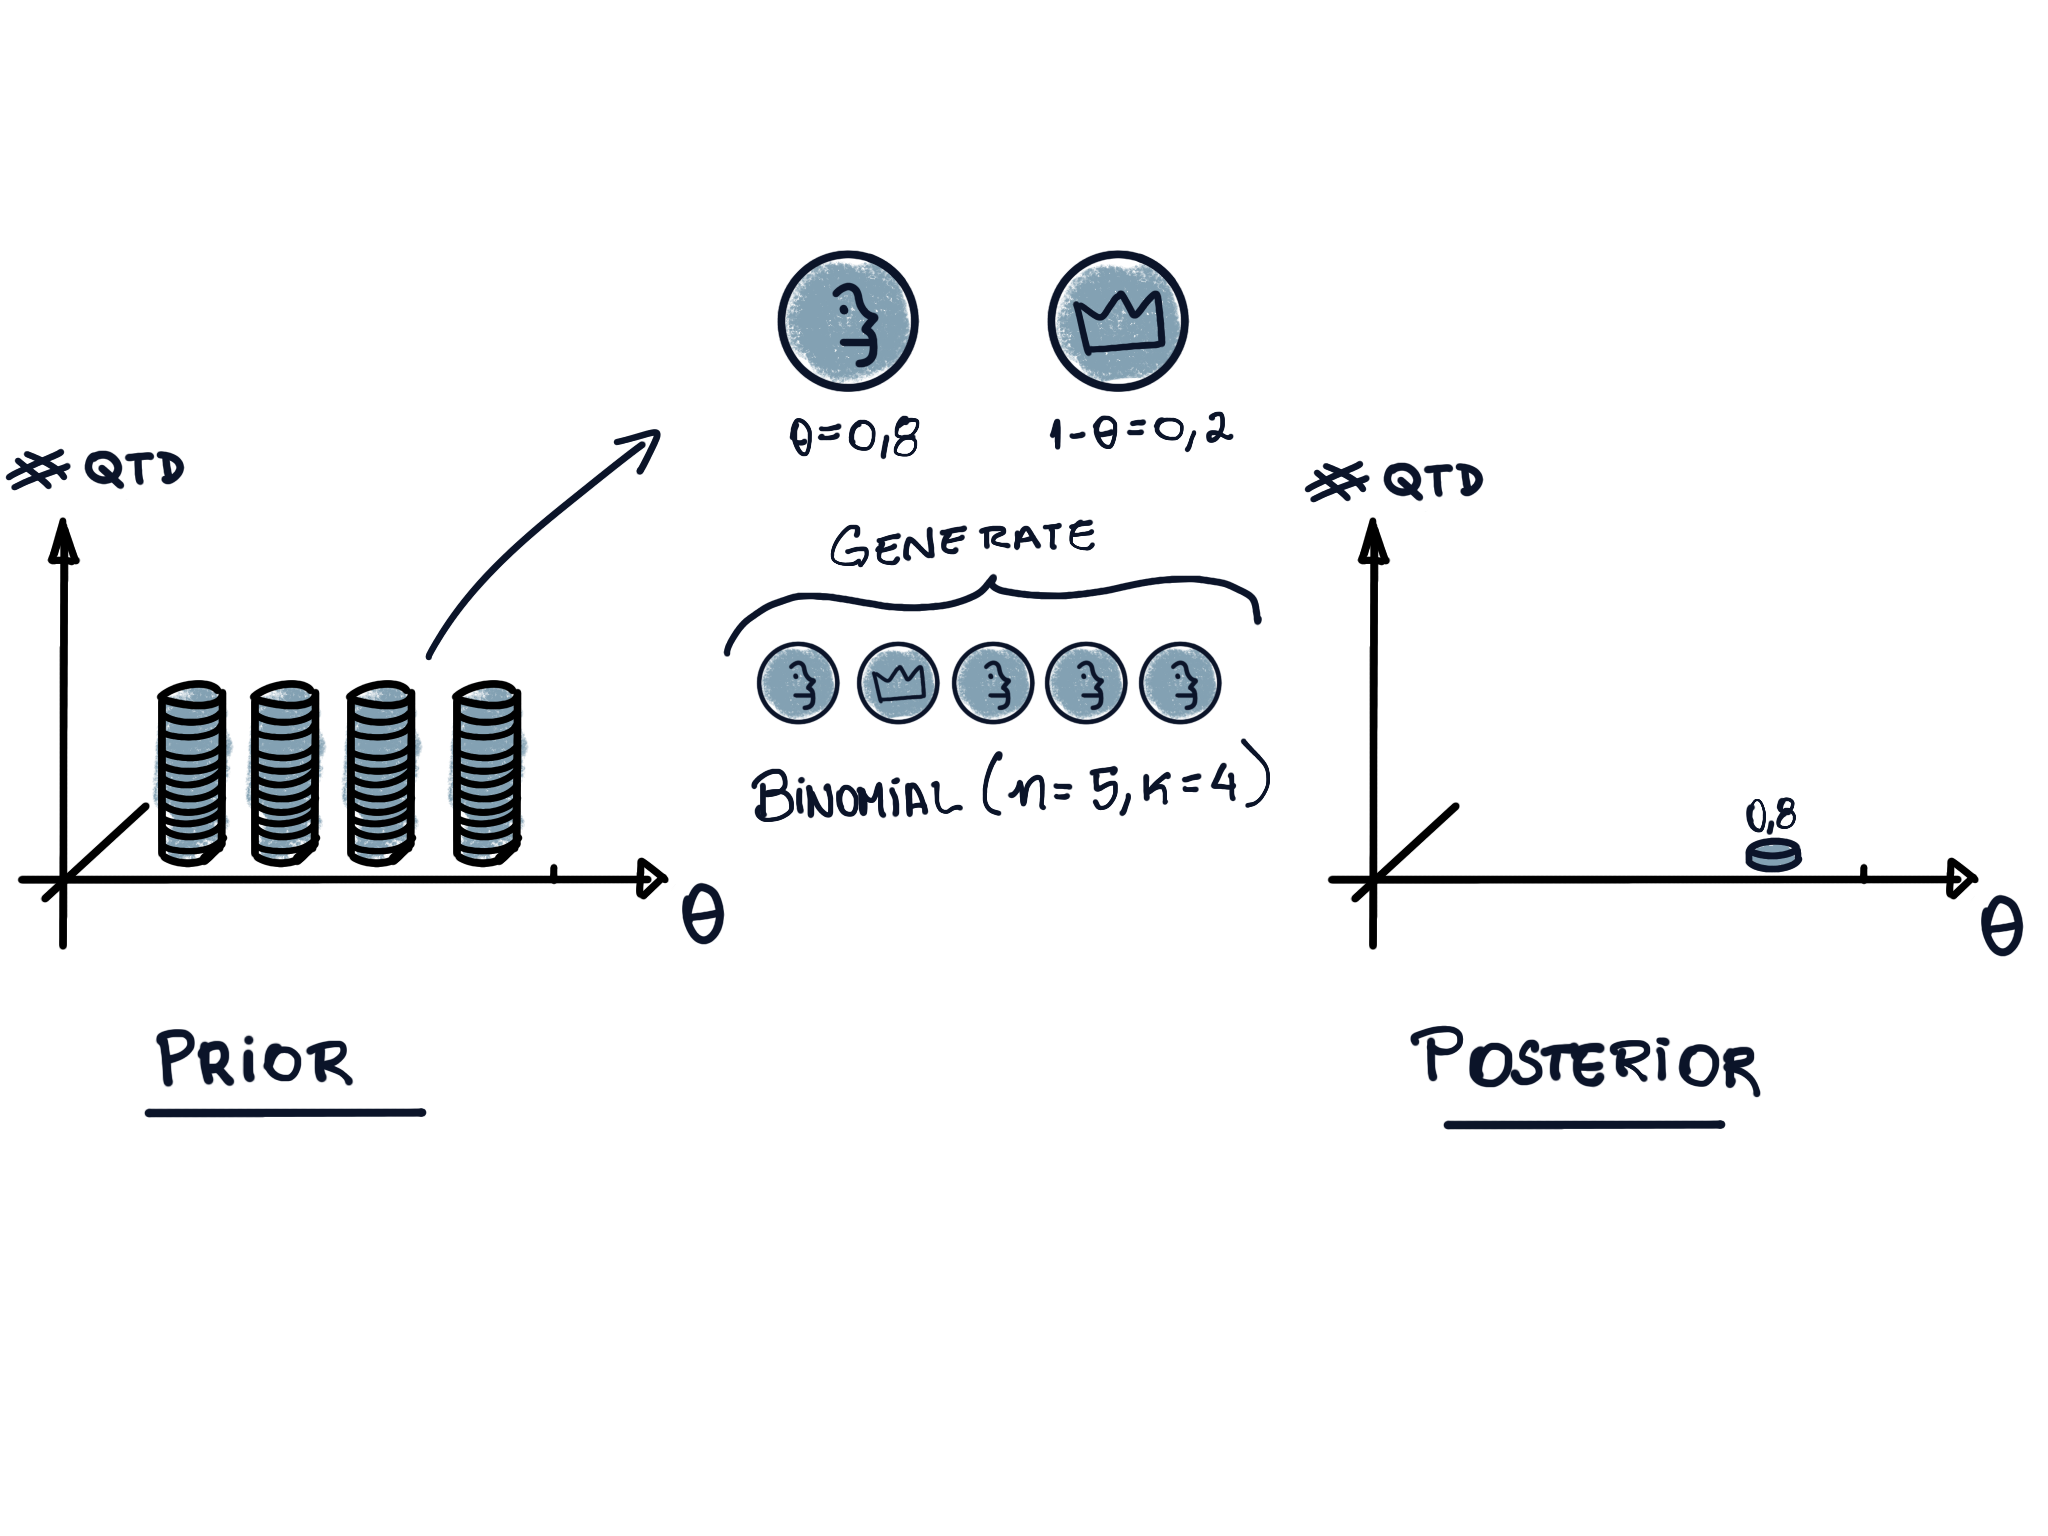
\includegraphics[width=10cm]{images/Vis-ABC.png}
        \caption{Schematic drawing of ABC method for Beta/Binomial
        model}
    \end{figure}

\end{frame}

\begin{frame}[fragile]{Original ABC Algorithm}

  The proof that the algorithm indeed results in an iid sample
  from the posterior is shown below. Let $\bm y$ be the observed,
  $\bm \theta$ the parameter of interest and $\bm z$ the generated
  samples.
  $$
  p(\bm \theta_i) \propto \sum_{\bm z \in \mathbb{D}}
  \pi(\bm \theta_i) p(\bm z \mid \bm \theta_i) \mathbb I_{\bm y}(\bm z)
  = \pi(\bm \theta_i) p(\bm y \mid \bm \theta_i) \propto
  \pi(\bm \theta_i \mid \bm y)
  $$

\end{frame}

\begin{frame}[fragile]{Original ABC Algorithm}

  \citet{Pritchard1999} extended the original algorithm to the case
  of continuos sample spaces.

  \vspace{0.3cm}

\begin{algorithm}[H]
\SetAlgoLined
\For{i=1 to N}{
 \Repeat{$\rho[\eta(\bm y) , \eta (\bm z)] \leq \epsilon$}{
    Sample $\bm\theta' \sim \pi(\cdot)$

    Generate $\bm z \sim p(\cdot \mid \bm\theta')$
 }
  
}
 \caption{ABC method for discrete and continuous distributions}
\end{algorithm}
\begin{itemize}
  \item[--] $\eta$: function defining a statistic (e.g. the mean),
  \item[--] $\rho$: a distance function,
  \item[--] $\epsilon$: acceptance tolerance.
\end{itemize}

\end{frame}

\begin{frame}[fragile]{Original ABC Algorithm}

  For this ABC algorithm, instead of the actual posterior,
  we get
  $$
  \pi_\epsilon(\bm \theta, \bm z \mid \bm y) = 
  \frac{\pi(\bm \theta) p(\bm z \mid \bm \theta)
  \mathbb I_{A_{\epsilon,\bm y}}(\bm z)}
  {\int_{A_{\epsilon,\bm y}\times \bm\theta}\pi(\bm \theta)
  p(\bm z \mid \bm \theta)d\bm z d \bm \theta}
  $$
  Where, $A_{\epsilon,\bm y} = \{
  \bm z \in \mathbb D \mid \rho[\eta(\bm z), \eta(\bm y) \leq \epsilon].
  \}$

  Hence, for a tolerance ($\epsilon$) "small enough", we expect a good
  approximation.
  $$\pi_\epsilon(\bm \theta \mid \bm y) = 
  \int \pi_\epsilon(\bm \theta, \bm z \mid \bm y) d \bm z \approx
  \pi(\bm \theta \mid \bm y)$$

\end{frame}

\AtBeginSection{}
\section[Moving Average]{Moving Average}
\begin{frame}[fragile]{Moving Average}

  We will use the Moving Average model, also denoted as MA(q),
  for assessing the performance of the ABC methods. The MA(q) process
  is a stochastic process defined by:
  $$y_k = u_k + \sum_{i=1}^q \theta_i u_{k-i}$$
  Where $(u_k)_{k \in \mathbb Z} \overset{iid}{\sim} N(0,1)$.
  For a $q=2$, imposing the standard identifiability condition
  we obtain the following conditions:
  $$
  -2 < \theta_1 < 2, \quad \quad \theta_1+\theta_2 > -1, \quad \quad
  \theta_1 - \theta_2 < 1.
  $$
  Hence, we use an uniform distribution over this triangular region as
  prior for $\bm \theta$. The likelihood of $\bm y \mid \bm \theta$ is
  more complex because of the need to integrate $\bm u$.

\end{frame}

\begin{frame}[fragile]{Moving Average}
  
  We generate a synthetic sample of length 100 using
  $(\theta_1, \theta_2) = (0.6, 0.2)$. For $q=2$ we can also
  numerically calculate the real posterior and the marginal distributions.

  $$
  \pi(\bm\theta \mid \bm y) \propto \pi(\bm\theta)
  p(\bm y \mid \bm \theta), \quad \quad
  \bm y \mid \bm \theta \sim MVN(0, \Sigma) \quad
  $$

  $$
  \Sigma =
  \tiny{
  \begin{bmatrix}
   1+\theta_1^2 + \theta_2^2    & \theta_1 + \theta_2 \theta_1 & \theta_2                     & 0                            & 0        & 0 & ... & 0 \\
   \theta_1 + \theta_2 \theta_1 & 1+\theta_1^2 + \theta_2^2    & \theta_1 + \theta_2 \theta_1 & \theta_2                     & 0        & 0 & ... & 0 \\
   \theta_2                     & \theta_1 + \theta_2 \theta_1 & 1+\theta_1^2 + \theta_2^2    & \theta_1 + \theta_2 \theta_1 & \theta_2 & 0 & ... & 0 \\
   0               & \theta_2   & \theta_1 + \theta_2 \theta_1 & 1+\theta_1^2 + \theta_2^2    & \theta_1 + \theta_2 \theta_1 & \theta_2 &... & 0 \\
   \vdots & \vdots & \vdots & \vdots & \vdots & \vdots & \vdots & \vdots \\
   0 & 0 & 0 & 0 & 0 & \theta_2 & \theta_1 + \theta_1\theta_2 & 1+\theta_1^2 + \theta_2^2 \\
  \end{bmatrix}}
  $$

\end{frame}

\begin{frame}[fragile]{Moving Average}

  For this model, the ABC algorithm consists of:
  \begin{itemize}
    \item Sample $\bm \theta ^ *$ from the uniform triangular prior
    using rejection sampling;
    \item For each $k \in \{-1,0, 1, ..., 100 \}$, sample
    $u_k \overset{iid}{\sim} N(0,1)$.
    \item For each $k \in \{ 1, 2, ..., 100\}$, calculate 
    $z_k = u_k + \sum^2_{i=1}\theta_i^* u_{k-i}$.
  \end{itemize}

  Two distance metrics are used. The raw distance between the series
  $$
  \rho^2\{ \bm z, \bm y\} = \sum^{n=100}_{k=1}(y_k - z_k)^2
  $$
  And the sum of the quadratic distances between the first $q = 2$
  autocovariances
  $$
  \tau_j(\bm x) = \sum^{n=100}_{k = j+1} x_k x_{k-j}, \quad \quad
  \rho^2 = \sum^{q=2}_{j=0}(\tau_j(\bm y) - \tau_j(\bm z))^2
  $$

\end{frame}

\begin{frame}[fragile]{Moving Average}

  Below we present the results of running ABC for the MA(2) process.
    \begin{figure}[H]
        \centering
        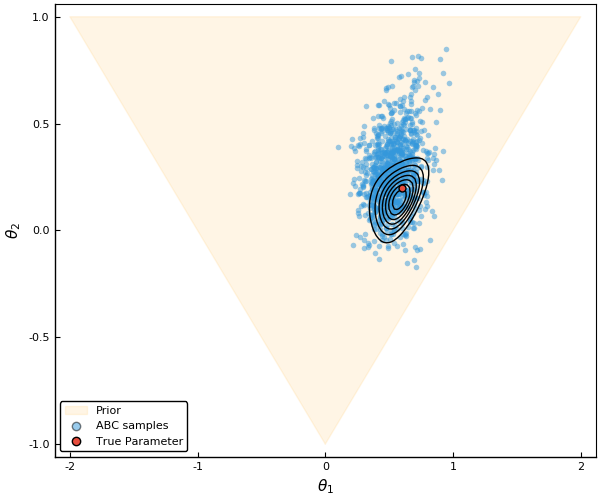
\includegraphics[width=6cm]{images/ABCmodel1.png}
        \caption{Comparison between the true posterior
        (\textit{line in black}), with the samples produced using the ABC
        . The number of simulations is $N = 10^6$,
        and the threshold $\epsilon$ corresponds to the quantile of
        accepting 0.1\%. The $\rho$ used was the distance
        of the autocovariances.}
    \end{figure}

\end{frame}

\AtBeginSection{}
\section[Calibration]{Calibration of ABC}
\begin{frame}[fragile]{Calibration of ABC}
  \textbf{Summary Statistics}($\eta$). As the number of observations
  grow, using the raw distance between each observation becomes too
  prohibitive. The alternative is to try using summary statistics,
  if possible, sufficient statistics.

  \citet{fearnhead2010constructing} created a way of constructing
  appropriate summary statistics for ABC in a semi-automatic manner.

  \textbf{Tolerance threshold}. The standard practice is to use 
  $\epsilon$  as a quantile of the simulated distances.

\end{frame}

\begin{frame}[fragile]{Calibration of ABC}

    \begin{figure}[H]
        \centering
        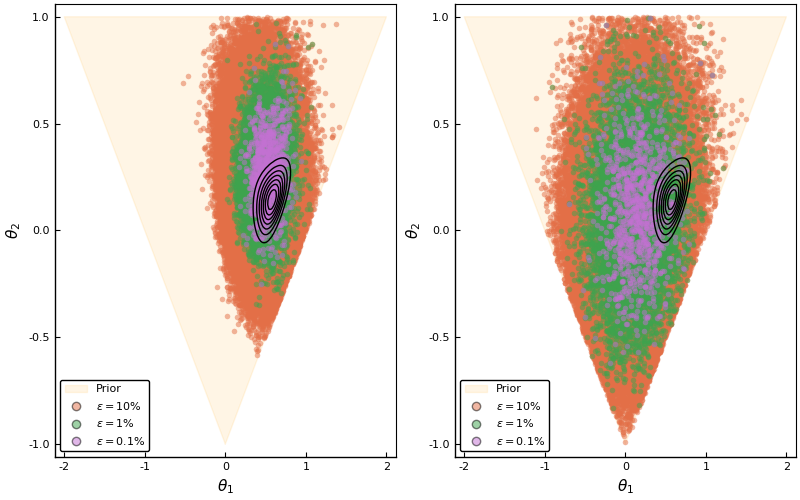
\includegraphics[width=9cm]{images/ABCmodel1_Comparison.png}
        \caption{Comparison of ABC method when using autocovariance
        distance 
\footnote{in the rest of the slides we will
        only use the autocovariance distances}
        (\textit{left}) versus raw distance (\textit{right}).
        The number of simulations is $N = 10^6$ and different
        thresholds $\epsilon$ are used.}
    \end{figure}

\end{frame}

\begin{frame}[fragile]{Calibration of ABC}

    \begin{figure}[H]
        \centering
        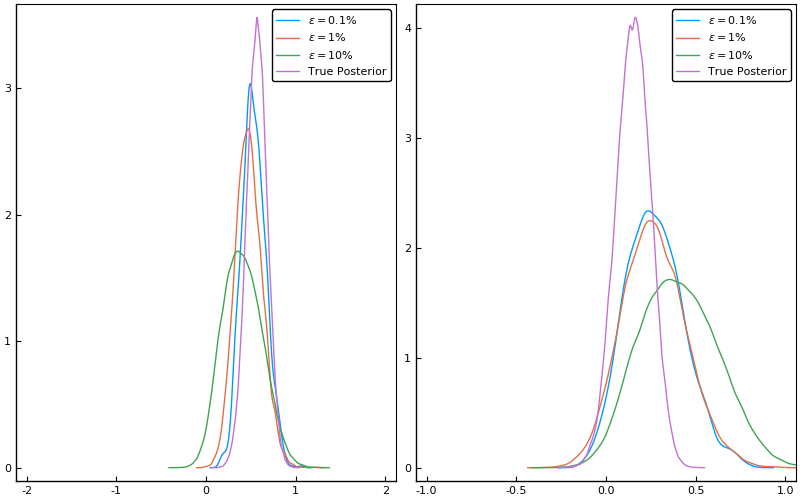
\includegraphics[width=9cm]{images/ABCmodel1_Marginal.png}
        \caption{Comparison of ABC samples with the true posterior
        marginal distribution for $\theta_1$ (\textit{left}) and
        $\theta_2$ (\textit{right}).
        }
    \end{figure}

\end{frame}

\AtBeginSection{}
\section[ABC Variations]{ABC Variations}
\begin{frame}[fragile]{ABC Variations}
  Using non-informative priors is usually very inefficient,
  because it leads to lots of rejections. To tackle this
  problem, \citet{Marjoram2013} came up with MCMC-ABC.


\footnotesize
\begin{algorithm}[H]
\SetAlgoLined
Use Algorithm 2 to get $(\bm \theta^{(0), \bm z^{(0)}}$ from the
target $\pi_\epsilon(\bm \theta, \bm z \mid \bm y)$.

\For{i=1 to N}{
 \Repeat{$\rho[\eta(\bm y) , \eta (\bm z)] \leq \epsilon$}{
    Sample $\bm\theta'$ from the Markov kernel
    $q(\cdot \mid \theta^{(i-1)})$

    Generate $\bm z \sim p(\cdot \mid \bm\theta')$

    Sample $u \sim U[0,1]$

    \If{
      $u \leq \frac{
                    \pi(\bm\theta')q(\bm\theta^{(i-1)}\mid)}
          {\pi(\bm\theta^{(i-1)})q(\bm\theta^{(i-1)}\mid)}$ and
      $\rho\{ \eta(\bm z'),\eta(\bm y) \} \leq \epsilon$
    }
    {Set $(\bm \theta^{(i)}, \bm z^{(i)}) =
    (\bm \theta', \bm z')$}
    % \If{$u \leq \frac{
    % \pi(\bm\theta')q(\bm\theta^{(i-1)}\mid)}
    % {\pi(\bm\theta^{(i-1)})q(\bm\theta^{(i-1)}\mid)}$}
    % }
    \Else
    {Set $(\bm \theta^{(i)}, \bm z^{(i)}) =
    (\bm \theta^{(i-1)}, \bm z^{(i-1)})$}
}
}
 \caption{MCMC-ABC}
\end{algorithm}
\end{frame}

\begin{frame}[fragile]{ABC Variations}

    \begin{figure}[H]
        \centering
        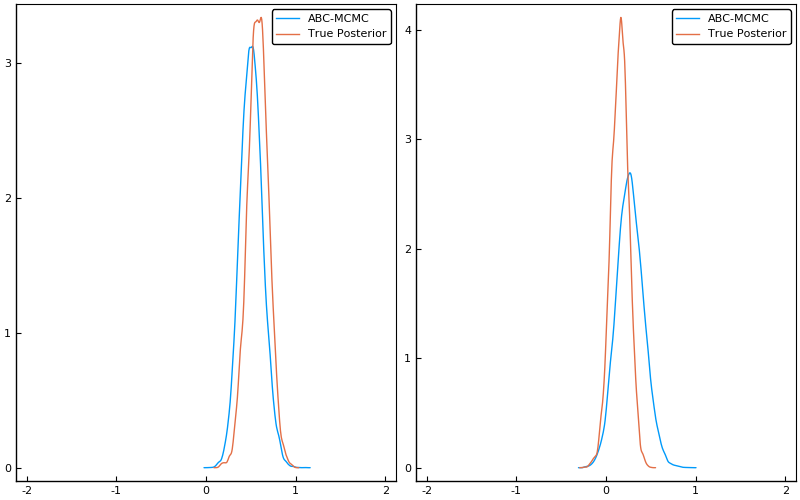
\includegraphics[width=9cm]{images/ABC-MCMC.png}
        \caption{Comparison of ABC-MCMC samples with the true posterior
        marginal distribution for $\theta_1$ (\textit{left}) and
        $\theta_2$ (\textit{right}) using $\epsilon = 0.1\%$.
        }
    \end{figure}

\end{frame}

\begin{frame}[fragile]{ABC Variations}

  Another variation of ABC is called \textit{Noisy} ABC, that was
  proposed by \citet{Wilkinson2013}. The original ABC algorithm can
  be thought as a rejection algorithm using a uniform kernel
  ($\mathbb I_{A_{\epsilon, \bm y}(\bm z)}$). The \textit{Noisy} version
  generalizes this, allowing the use of different kernels, hence:
  $$
  \pi_\epsilon(\bm \theta, \bm z \mid \bm y) = 
  \frac{\pi(\bm \theta) p(\bm z \mid \bm \theta)
  K_\epsilon(\bm y - \bm z)}
  {\int \pi(\bm \theta)
  p(\bm z \mid \bm \theta)K_\epsilon(\bm y - \bm z)d\bm z d \bm \theta}
  $$

  Now, instead of accepting if
  $\rho\{\eta(\bm y),\eta(\bm z)\} \leq \epsilon$, we accept with 
  probability
  $\frac{K_\epsilon(\bm y - \bm z)}{max\{K_\epsilon(\bm y - \bm z\})}
  $.

\end{frame}

\begin{frame}[fragile]{ABC Variations}

    \begin{figure}[H]
        \centering
        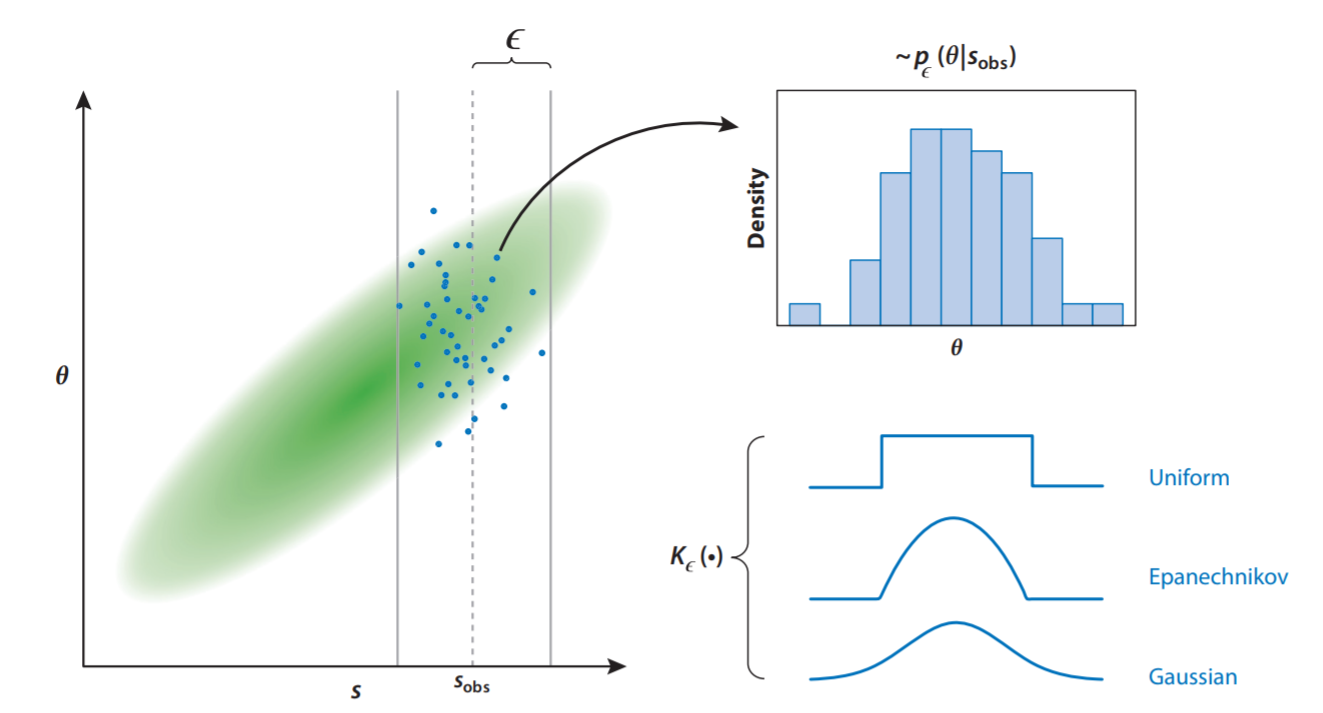
\includegraphics[width=9cm]{images/NoisyABC.png}
        \caption{
        Illustration of \textit{Noisy} ABC rejection kernels, where
        $s$ is the statistic from the ABC sampler and $s_{obs}$ is 
        the observed value from the data.
        Figure from \cite{Beaumont2018}.
        }
    \end{figure}

\end{frame}

\begin{frame}[fragile]{ABC Variations}

  Sequential techniques are also used with ABC to enhance the
  efficiency of the algorithms. A popular method in this regard is
  the ABC-PMC (ABC population Monte Carlo) by \citet{Beaumont2009}.
  It estimates the scale of the random walk step from the previous
  simulations and
  uses a sequence of tolerance thresholds
  ($\epsilon_1 \geq ... \geq \epsilon_T$) to approximate the distribution.

   A recent work by \citet{Simola2019} propose a method
   for adaptively selecting this sequence of tolerances that
   improves computationla efficiency and defines a stopping rule,
   thus assisting in automating the termination of the sampling
   procedure.
\end{frame}

\begin{frame}[fragile]{ABC Variations}

    \begin{figure}[H]
        \centering
        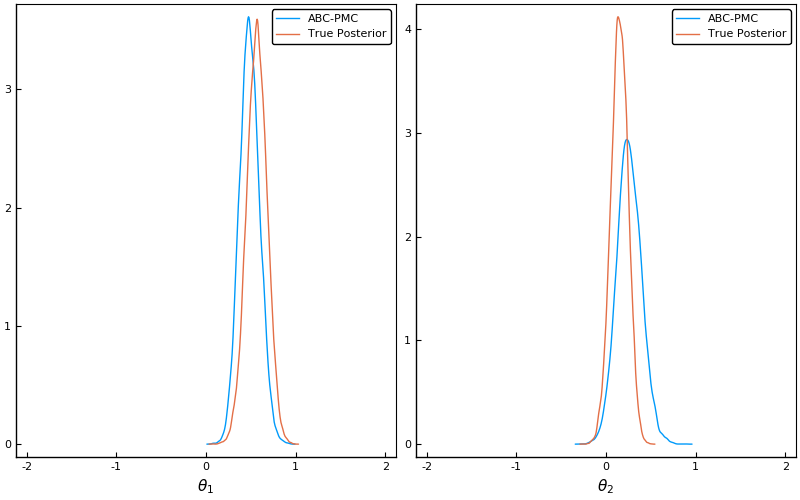
\includegraphics[width=9cm]{images/ABC-PMC.png}
        \caption{Comparison of ABC-PMC samples with the true posterior
        marginal distribution for $\theta_1$ (\textit{left}) and
        $\theta_2$ (\textit{right}) using $\epsilon = 0.1\%$.
        }
    \end{figure}

\end{frame}
% \appendix
\AtBeginSection{}
\section[Post-Processing of ABC]{Post-processing of ABC}
\begin{frame}[fragile]{Post-processing of ABC}
  
  \textit{Local linear regression} was proposed by
  \citet{Beaumont2012} as a way improve the result of simulations
  without the need to use restrictively low threshold values.
  The idea is then to use a weighted least squares regression
  of $\bm \theta$ on $(\eta(\bm y) - \eta(\bm z))$, with weights
  according to a chosen kernel.
  $$
  \bm \theta^* = \bm \theta - (\eta(\bm y) - \eta(\bm z))^T\hat\beta
  $$

\end{frame}

\begin{frame}[fragile]{Post-processing of ABC}
  
    \begin{figure}[H]
        \centering
        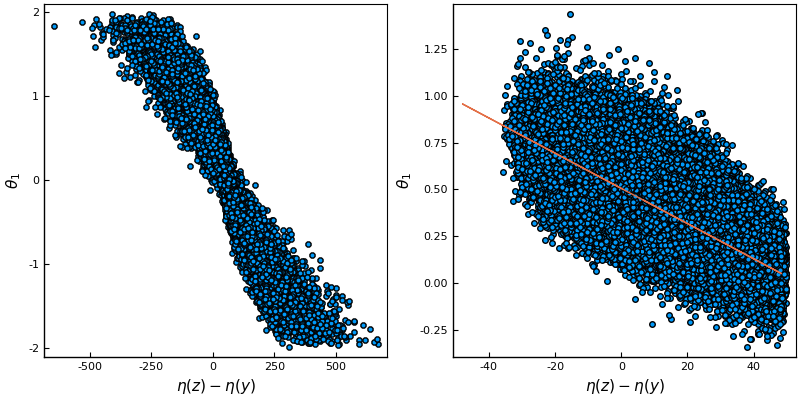
\includegraphics[width=9cm]{images/RegressionABC1.png}
        \caption{Scatter plots of simulated $\theta_1$ and
        $(\eta(\bm y)-\eta(\bm z))$ for autocovariance with
        $lag = 1$. On the \textit{left} there are all the
        $N=10^6$ simulations, while in the \textit{right} only the
        accepted samples for $\epsilon = 10\%$ with the regression
        line.
        }
    \end{figure}


\end{frame}

\begin{frame}[fragile]{Post-processing of ABC}

    \begin{figure}[H]
        \centering
        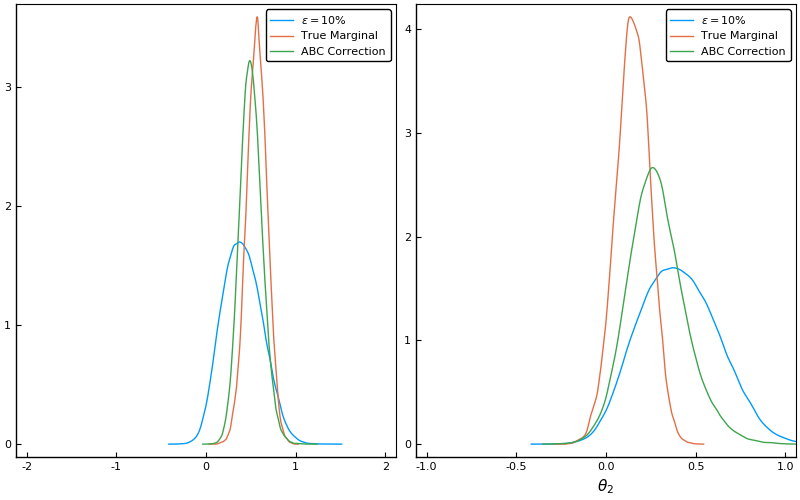
\includegraphics[width=9cm]{images/ABCRegression_Marginal.png}
        \caption{Comparison of ABC samples corrected through
        local linear regression versus the true marginal posterior
        distribution for $\theta_1$ (\textit{left}) and
        $\theta_2$ (\textit{right}) using $\epsilon = 10\%$.
        }
    \end{figure}

\end{frame}



\AtBeginSection{}
\section[Model Choice]{Model Choice}
\begin{frame}[fragile]{Model Choice}
  The estimation of the posterior using ABC is straightfoward.

  \begin{algorithm}[H]
  \SetAlgoLined
  \For{i=1 to N}{
    \Repeat{$\rho[\eta(\bm y) , \eta (\bm z)] \leq \epsilon$}{
      Sample $m \sim \pi(\mathcal{M}=m)$

      Sample $\bm\theta_m \sim \pi_m(\bm \theta_m)$

      Generate $\bm z \sim p_m(\cdot \mid \bm\theta_m)$
   }
   Set $m^{(i)}=m$ and $\bm\theta^{(i)} = \bm\theta_m$
    
  }
   \caption{ABC Model Choice}
  \end{algorithm}

  The posterior probability $\pi(\mathcal{M}=m \mid \bm y)$
  if the acceptance frequency from model m,
  $$
  \frac{1}{N}\sum^N_{i=1}\mathbb I_{m^{(i)}=m}
  $$


\end{frame}

\begin{frame}[fragile]{Post-processing of ABC}

    \begin{figure}[H]
        \centering
        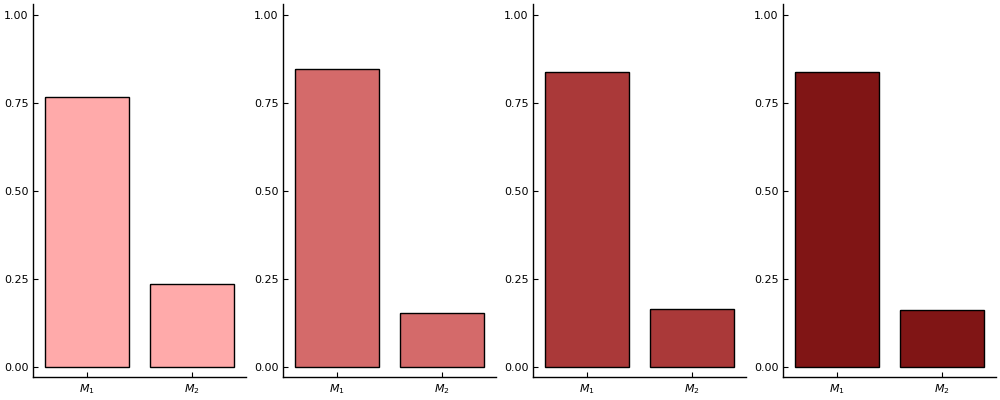
\includegraphics[width=11.2cm]{images/ModelChoice_MA2.png}
        \caption{Barplots of evolution of Bayes factor approximations
        in terms of visits to models MA(1) and MA(2) using
        ABC using thresholds of 10, 1, 0.1 , 0.01 \% on autocovariance
        distance. The true model is MA(2) and the true Bayes factor is 0.952.
        }
    \end{figure}

\end{frame}

\begin{frame}[fragile]{Post-processing of ABC}

    \begin{figure}[H]
        \centering
        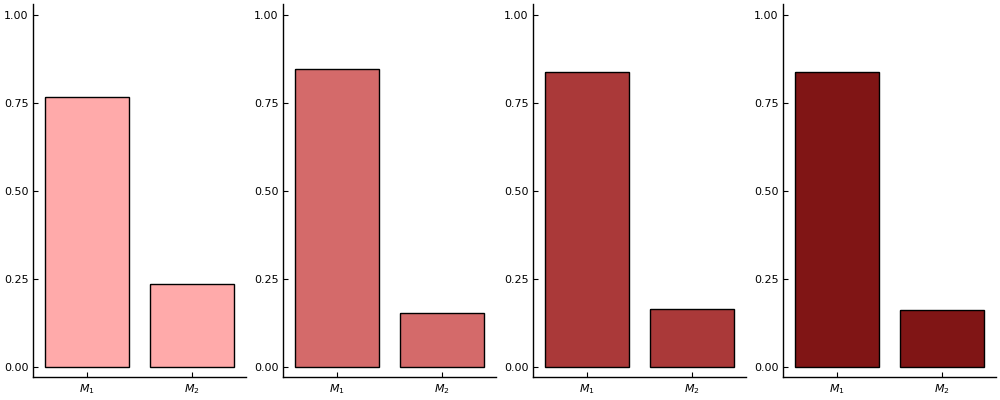
\includegraphics[width=11.2cm]{images/ModelChoice_MA1.png}
        \caption{Barplots of evolution of Bayes factor approximations
        in terms of visits to models MA(1) and MA(2) using
        ABC using thresholds of 10, 1, 0.1 , 0.01 \% on autocovariance
        distance. The true model is MA(1) and the true Bayes factor is 0.943.
        }
    \end{figure}

\end{frame}

\begin{frame}[allowframebreaks]{References}

% \renewcommand{\bibsection}{\section{}}
  \renewcommand{\section}[2]{}%
  \bibliography{abc}
  % \bibliographystyle{plainnat}
  % \bibliographystyle{plain}
  % \bibliographystyle{abbrv}
  \bibliographystyle{apa}

\end{frame}

\end{document}
